%%%%%%%%%%%%%%%%%%%%%%%%%%%%%%%%%%%%%%%%%%%%%%%%%%%%%%%%%%%%%%%%%
%%  To create image run: (for Windows use imgconvert)
%%
%%  convert -verbose -delay 50 -loop 0 -density 300 -resize 640x480 <name>.pdf <name>.gif
%%
%%%%%%%%%%%%%%%%%%%%%%%%%%%%%%%%%%%%%%%%%%%%%%%%%%%%%%%%%%%%%%%%
%%
%%  Modified from github.com/thetensor-space/Tenscenery
%%
%%%%%%%%%%%%%%%%%%%%%%%%%%%%%%%%%%%%%%%%%%%%%%%%%%%%%%%%%%%%%%%%
\documentclass[beamer,tikz,preview]{standalone}
%\documentclass{beamer}

\setbeamertemplate{navigation symbols}{}
\usefonttheme{professionalfonts} % using non standard fonts for beamer
\usepackage{tikz}
\usepackage{xcolor}
\usepackage{amssymb}
\usepackage{amsmath}

\begin{document}
\begin{frame}
    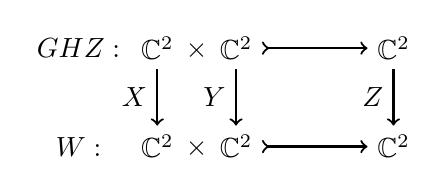
\begin{tikzpicture}
        % Pieces
        \node (GHZ) at (0, 1.25) {$GHZ:$};
        \node (W) at (0, 0) {$W:$};
        \node (U2) at (1, 1.25) {$\mathbb{C}^2$};
        \node (x1) at (1.5, 1.22) {$\times$};
        \node (U1) at (2, 1.25) {$\mathbb{C}^2$};
        \node (U0) at (4, 1.25) {$\mathbb{C}^2$};
        \node (V2) at (1, 0) {$\mathbb{C}^2$};
        \node (x2) at (1.5, -0.03) {$\times$};
        \node (V1) at (2, 0) {$\mathbb{C}^2$};
        \node (V0) at (4, 0) {$\mathbb{C}^2$};

        % Arrows
        \draw[>->, thick] (U1) -- (U0);
        \draw[>->, thick] (V1) -- (V0);
        \draw[->, thick] (U2) -- (V2) node[midway, left] {$X$};
        \draw[->, thick] (U1) -- (V1) node[midway, left] {$Y$};
        \draw[->, thick] (U0) -- (V0) node[midway, left] {$Z$};
    \end{tikzpicture}
\end{frame}

\end{document}